\documentclass[12pt, a4paper]{article}
\usepackage{ctex}
\usepackage{graphicx}
\usepackage{float}
\usepackage[super, square]{natbib}
\usepackage{booktabs}
\usepackage[margin = 1in]{geometry}
\usepackage{
  color,
  clrscode,
  amssymb,
  ntheorem,
  amsmath,
  listings,
  fontspec,
  xcolor,
  supertabular,
  multirow
}
\renewcommand\contentsname{Contents}
\renewcommand\refname{References}
\renewcommand\figurename{Fig.}
\definecolor{bgGray}{RGB}{36, 36, 36}
\usepackage[
  colorlinks,
  linkcolor=bgGray,
  anchorcolor=blue,
  citecolor=black
]{hyperref}
\newfontfamily\courier{Courier}

\theoremstyle{margin}
\theorembodyfont{\normalfont}

\newtheorem{theorem}{Theorem}
\newtheorem{definition}[theorem]{Definition}
\newtheorem{example}[theorem]{Example}

\newcommand{\st}{\text{s.t.}}
\newcommand{\mn}{\mathnormal}
\newcommand{\tbf}{\textbf}
\newcommand{\fl}{\mathnormal{fl}}
\newcommand{\f}{\mathnormal{f}}
\newcommand{\g}{\mathnormal{g}}
\newcommand{\R}{\mathbf{R}}
\newcommand{\Q}{\mathbf{Q}}
\newcommand{\JD}{\textbf{D}}
\newcommand{\rd}{\mathrm{d}}
\newcommand{\str}{^*}
\newcommand{\vep}{\varepsilon}
\newcommand{\lhs}{\text{L.H.S}}
\newcommand{\rhs}{\text{R.H.S}}
\newcommand{\con}{\text{Const}}
\newcommand{\oneton}{1,\,2,\,\dots,\,n}
\newcommand{\aoneton}{a_1a_2\dots a_n}
\newcommand{\xoneton}{x_1,\,x_2,\,\dots,\,x_n}

\title{Project Report of RISC-V CPU\\\begin{large}Course Project of MS108 Computer System(1)\end{large}}
\author{Bohan Hou (侯博涵)\\ACM honor class @ Shanghai Jiao Tong University}
\date{}

\begin{document}

\lstset{numbers=left,
  basicstyle=\scriptsize\courier,
  numberstyle=\tiny\courier\color{red!89!green!36!blue!36},
  language=C++,
  breaklines=true,
  keywordstyle=\color{blue!70},commentstyle=\color{red!50!green!50!blue!50},
  morekeywords={},
  stringstyle=\color{purple},
  frame=shadowbox,
  rulesepcolor=\color{red!20!green!20!blue!20}
}
\maketitle

\section{Introduction}

GitHub repository of my CPU project: \url{https://github.com/spectrometerHBH/Chaos}

This project is a RISC-V CPU with Dynamic Sceduling and SuperScalar implemented in Verilog HDL, which is runnable on FPGA(tested on xc7a35t).

\section{Design}

\subsection{Features}

Main features of this RISC-V CPU are briefly introduced in the table below.

\begin{table}[H]
\centering
\begin{tabular}{@{}ll@{}}
\toprule
\multicolumn{1}{c}{Feature} & \multicolumn{1}{c}{RISC-V CPU}                                                                        \\ \midrule
ISA                         & RISC-V RV32I subset\\
Clock Rate                  & 100MHz \\
UART                        & Baudrate 115200 bit/s \\
Pipelining                  & 3 stages(Fetch, Decode, Execution) \\
Dynamic Sceduling           & Tomasulo Algorithm \\
Superscalar                 & Multiple Issues(2 issues per clock at most) and FUs \\
Cache                       & 512B 2-way associative I-cache\\
Memory                      & 128K BRAM memory on chip \\ 
Branch Policy               & stall \\
\bottomrule
\end{tabular}
\end{table}

\subsection{Design Graph}

\begin{figure}[H]
	\begin{center}
	  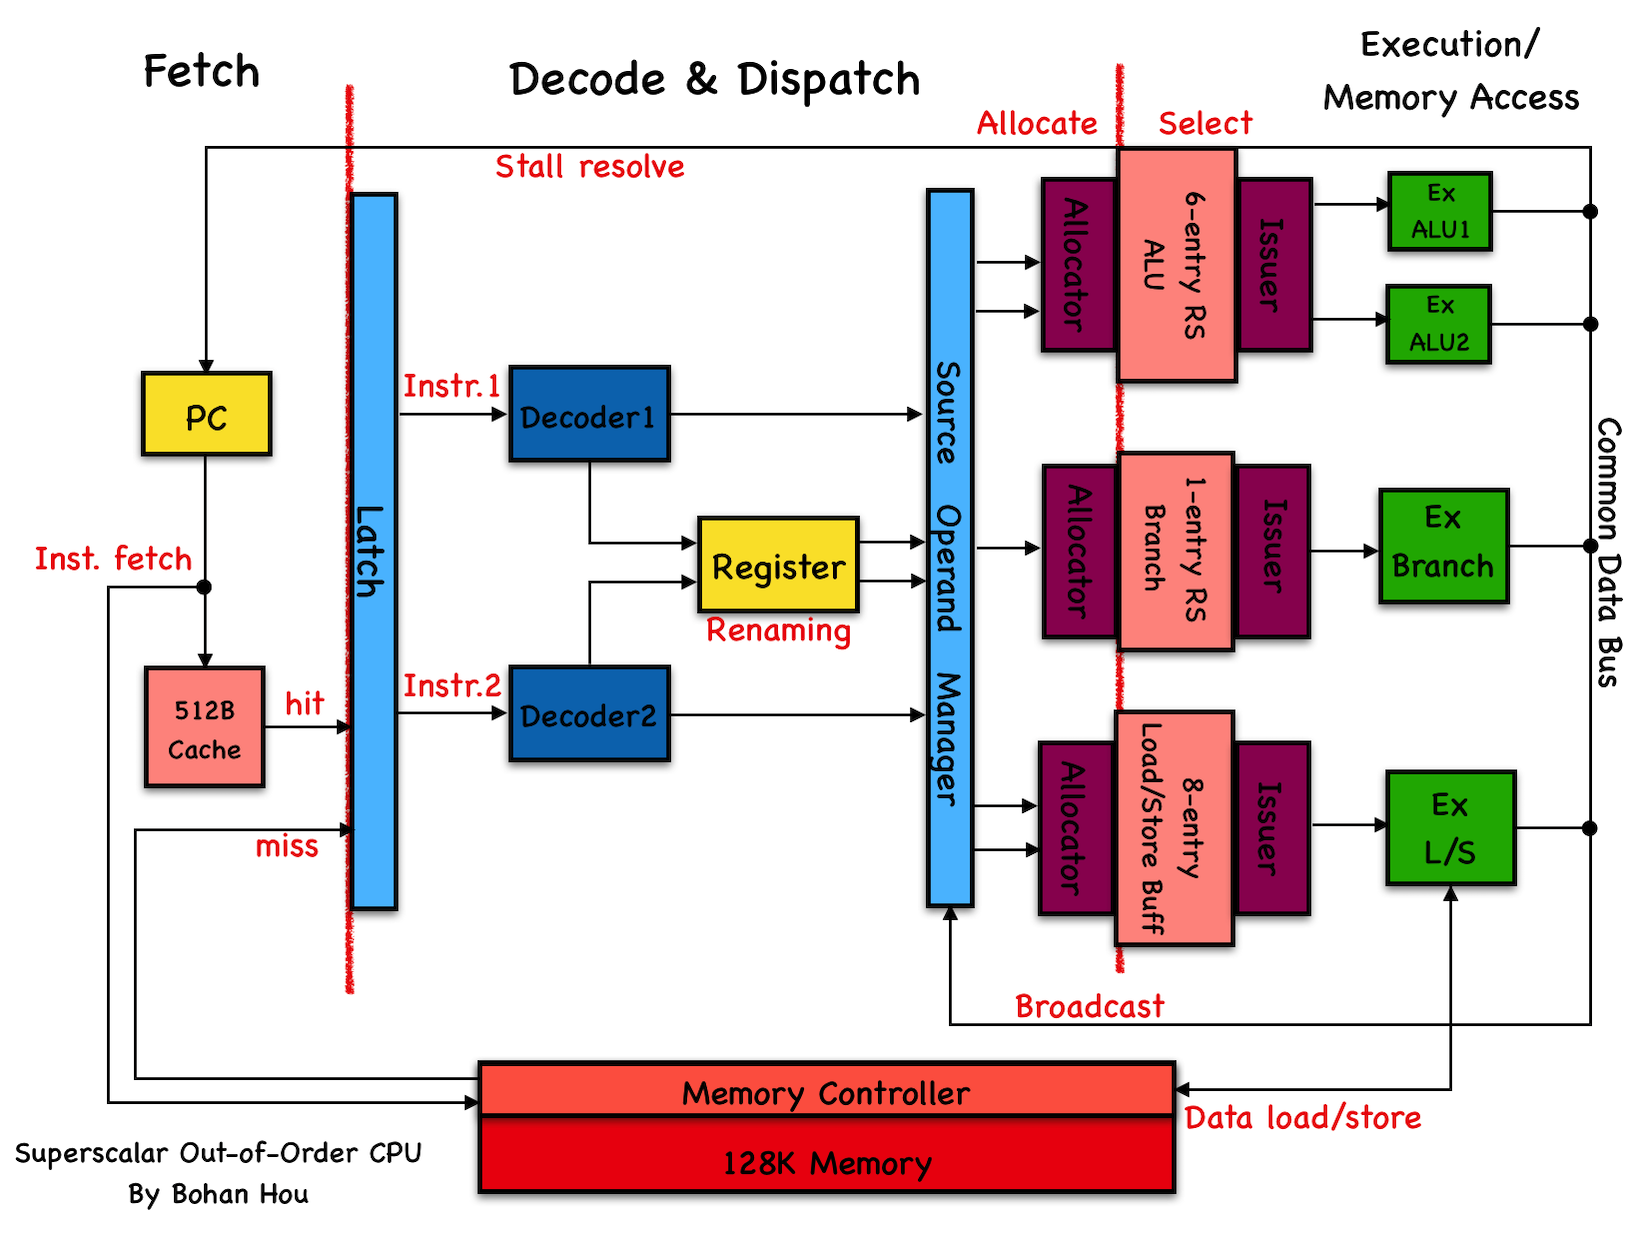
\includegraphics[height=9cm]{structure.png}
	\end{center}
	\caption{Overview of CPU Design}
\end{figure}

\subsection{Specification}
\begin{itemize}
  \item Fetch - Fetcher module sends signal to cache and memctrl at the same time. $T_{hit}$ = 1, $T_{penalty} \leq 15$ 
        If PC and PC+4 both hit in cache, Fetcher will send 2 instructions to Decode stage. 
        Fetcher will stall PC when branching or jumping. 
  \item Decode - Decoder and Dispatcher will decode the 2 instructions and allocate 2 locks to each of them. 
                 Dispatcher will address the dependence between the two instructions. 
  \item Execution - ALU reservation station will send at most 2 instructions to Execution stage.                
\end{itemize}

\begin{thebibliography}{9}
  \bibitem{caaqa} 
	John L. Hennessy, David A. Patterson, et al.
	\emph{Computer Architecture: A Quantitative Approach},
	Sixth Edition, 2019.
  \bibitem{ridecore}
  Arch Lab. in Tokyo Institute of Technology
  \emph{\href{https://github.com/ridecore/ridecore}{RIDECORE (RIsc-v Dynamic Execution CORE)}}
  
\end{thebibliography}

\end{document}
